

Razvijeni model za prijenos stila glazbe sastoji se od 3 komponente:
\begin{itemize}
  \item Okosnica Riffusion 
  \item Koder teksta iz CLIP-a
  \item Modul TVE (\textit{engl. Time - Varying Encoder})
\end{itemize}

\subsection{Okosnica Riffusion}
Model Riffusion\cite{forsgren2022riffusion} dizajniran je za rad sa spektrogramima zvuka za zadatke poput generiranja i transformacije glazbe. Sami model spada u latentne difuzijske modele (LDM), a na ulazu odnosno izlazu modela nalaze se mel-spektrogrami. Za zadani spektrogram na ulazu, model radi niz malih promjena (koraka uklanjanja šuma) sve dok (u ovom slučaju) spektrogram ne poprimi željeni stil. U našoj arhitekturi za prijenos stila glazbe, Riffusion se koristi kao okosnica sa zamrznutim parametrima.

\subsection{Koder teksta iz CLIP-a}
CLIP (engl. \textit{Contrastive Language–Image Pretraining})\cite{radford2021learning} model je strojnog učenja koji povezuje tekst i slike. Može se koristiti za povezivanje slika i pripadnih tekstualnih opisa, \textit{zero-shot} klasifikaciju, stvaranje opisa za slike i slično. Sastoji se od 2 dijela: kodera slika i kodera teksta. Koder slika ugrađuje slikovnu reprezentaciju u prostor ugrađivanja (latentni prostor), a koder teksta ugrađuje tekstualnu reprezentaciju u isti taj prostor ugrađivanja. U našoj arhitekturi za prijenos stila glazbe, koristi se samo predtrenirani koder teksta iz CLIP-a sa zamrznutim parametrima. 

\subsection{Modul TVE (\textit{engl. Time - Varying Encoder})}
Modul TVE ključna je inovacija u procesu prijenosa stila glazbe. Cilj je asocirati vremenski korak $t$ i ugrađivanje znaka "*" sa stilom tijekom učenja, kako bi se kasnije modul mogao koristiti u procesu prijenosa stila glazbe.

\begin{figure}[H]
    \centering
    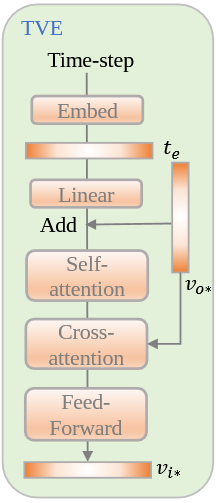
\includegraphics[width=0.5\linewidth]{imgs/tve.png}
    \caption{Arhitektura modula TVE. Preuzeto iz\cite{huang2024musicstyletransferdiffusion}.}
    \label{fig:arhitektura_tve}
\end{figure}


Na ulazu, modul prima vremenski korak $t$ i ugrađuje ga u prostor ugrađivanja sinusnim i kosinusnim transformacijama kao $t_{e}$. Zatim se vektor $t_{e}$ provede kroz 3 linearna sloja neuronske mreže uz aktivacijsku funkciju $SiLU$ nakon svakog sloja osim posljednjeg.

\begin{equation}
    SiLU({x}) = {x} \cdot \sigma({x})
\end{equation}

Nakon toga, vektoru $t_{e}'$ pribraja se ugrađivanje konstantnog znaka "*" $v_{o*}$ dobiveno pomoću kodera teksta iz CLIP-a. Dobiveno ugrađivanje $v_0$ zatim prolazi kroz sloj pažnje i sloj unakrsne pažnje. Oba sloja pažnje koriste \textit{dropout} iznosa 0.05 i imaju 8 glava pažnje. Jednadžba pažnje općenito je:

\begin{equation}
    {Attention}(Q, K, V) = softmax(\frac{QK^\top}{\sqrt{d}})\cdot V
\end{equation}

U ovom slučaju, ulaz u sloj pažnje je samo $v_0$, a ulaz u sloj unakrsne pažnje je $v_0$ i izlaz prvog sloja pažnje $v_1$.

\begin{align}
    v_1  &= {Attention}(v_0, v_0, v_0) \\
    v_i &= {Attention}(v_1, v_0, v_0)
\end{align}

Konačno, vektor prolazi kroz sloj \textit{dropout} iznosa 0.05 i još jedan linearni sloj te postaje vektor ugrađivanja $v_{i*}$. 

\subsection{Učenje modela}
Suradnju svih dosad opisanih dijelova arhitekture najbolje vidimo u procesu učenja, prikazanog na slici \ref{fig:arhitektura_train}. 

\begin{figure}[H]
    \centering
    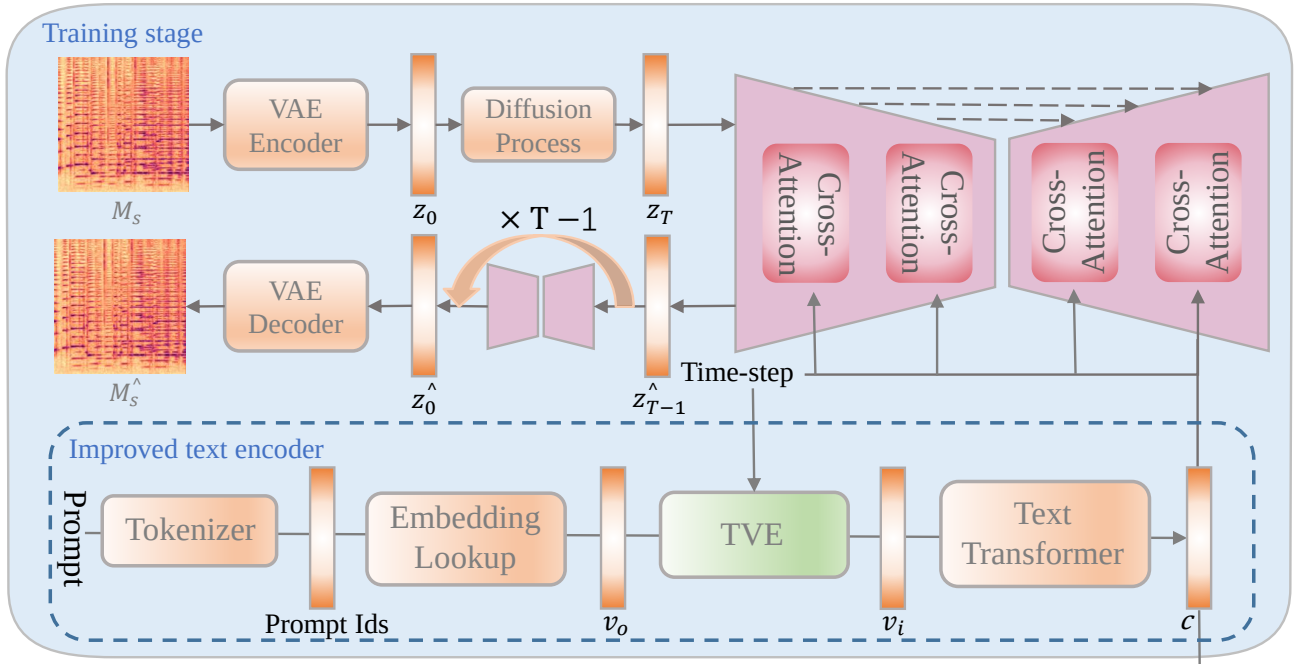
\includegraphics[width=0.9\linewidth]{imgs/train.png}
    \caption{Učenje modela. Preuzeto iz\cite{huang2024musicstyletransferdiffusion}.}
    \label{fig:arhitektura_train}
\end{figure}

Zadani mel-spektrogram stila prolazi kroz koder varijacijskog autoenkodera i prebacuje se u latentni vektor $z_0$. Zatim prolazi kroz difuzijski proces (\ref{eq:difusion}) od $T$ koraka i postaje zašumljeni latentni vektor $z_T$. Broj $T$  nasumično uzorkujemo u svakom koraku učenja.
\begin{equation}
    z_t = \sqrt{1 - \beta_t^2} \cdot z_{t-1} + \beta_t \cdot \epsilon_t
    \label{eq:difusion}
\end{equation}
Gdje je $0 < \beta_n^2 < 1$ i $\epsilon \sim N(0, 1)$.

Zašumljeni latentni vektor $z_T$ koristi se kao ulaz za model UNet koji sadrži slojeve unakrsne pažnje. Cilj je rekonstruirati vektor $\hat{z}_{T-1}$ iz vektora $z_T$ uklanjanjem šuma. Za predviđanje šuma u trenutku $T$, UNet osim zašumljenog latentnog vektora $z_T$ koristi i izlaz ranije opisanog modula TVE, koji na ulazu prima vremenski korak $T$ i ugrađivanje znaka "*" (dobivenom koristeći CLIP-ov tekstualni koder). 
  
Ovime je opisan jedan korak obrnute difuzije tj. uklanjanja šuma. Postupak se ponavlja za svaki korak $t$ sve dok ne dođemo do koraka $t = 0$ i latentnog prikaza $\hat{z}_0$:

\begin{equation}
    \hat{z}_{t-1} = f(\hat{z_t}, t, e_\theta(y, t))
\end{equation}

Pritom $e_\theta(y, t)$ označava izlaz modula TVE za zadano tekstualno ugrađivanje $y$ i korak $t$. Ovo ugrađivanje zovemo ugrađivanje stila za korak $t$.

Gubitak (\ref{eq:loss}) je definiran kao kvadrat L2 norme razlike stvarnog slučajnog šuma $\epsilon$ i šuma predviđenog modelom UNet $\epsilon_\phi$. 

\begin{equation}
    \mathcal{L} = \| \epsilon_t - \epsilon_\phi(z_t, t, e_\theta(y, t)) \|_2^2 ,
    \label{eq:loss}
\end{equation}

Dakle, uče se samo parametri $\theta$ modula TVE, dok su svi ostali parametri $\phi$ zamrznuti. Cilj optimizacije (utemeljen na prikazanom gubitku LDM-a) je:

\begin{equation}
    \theta^{*} = \arg\min_{\theta} \mathbb{E}_{z, y, \epsilon_t, t} \left[ \| \epsilon_t - \epsilon_\phi(z_t, t, e_\theta(y, t)) \|_2^2 \right],
\end{equation}

Drugim riječima, cilj je pronaći parametre $\theta^{*}$ modula TVE za koje je očekivanje kvadrirane L2 norme razlike stvarnog slučajnog šuma $\epsilon_t \sim N(0, 1)$ i predviđenog šuma modela $\epsilon_{\phi}$ minimalno.


\subsection{Prijenos stila}
Nakon što smo naučili modul TVE na željenom stilu, prenosimo ga procesom stilizacije reducirane pristranosti (engl. \textit{bias-reduced stylization}), prikazanom na slici \ref{fig:inference}. Cijeli proces sastoji se od tri glavna koraka.

\begin{figure}[H]
    \centering
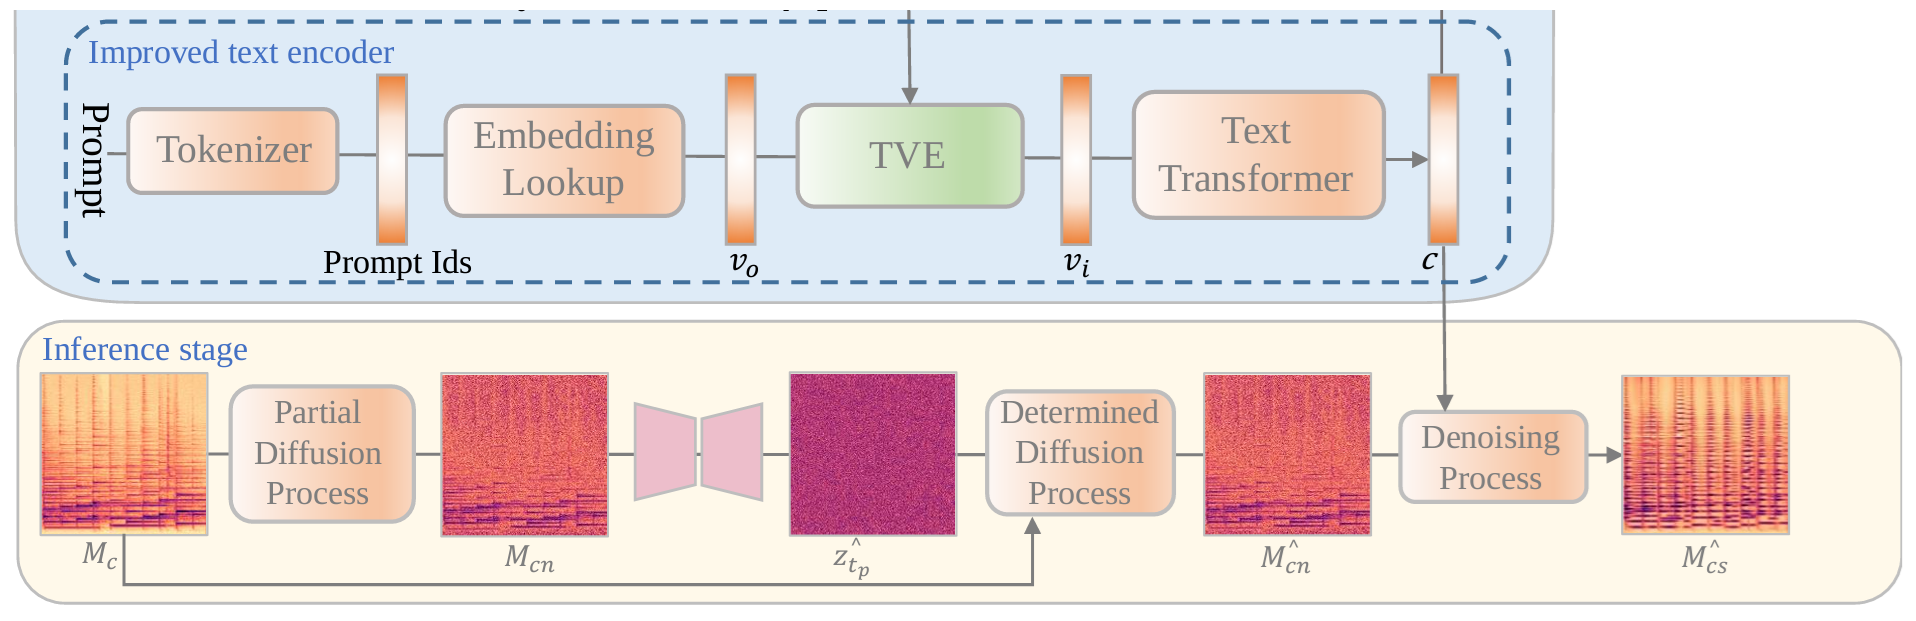
\includegraphics[width=0.9\linewidth]{imgs/inference.png}
    \caption{Prijenos stila. Preuzeto iz\cite{huang2024musicstyletransferdiffusion}.}
    \label{fig:inference}
\end{figure}

Prvi korak prijenosa stila je parcijalni proces difuzije. Mel-spektrogramu $M_c$ (koji predstavlja glazbu na koju želimo prenijeti stil), u latentnom prostoru VAE-a, prvo se difuzijskim procesom dodaje šum dok ne dođe do koraka $t_p = T \cdot strength$. Zašumljeni latentni vektor spektrograma u koraku $t_p$ označavamo s $M_{cn}$. 
  
Nakon prvog koraka prijenosa stila slijedi korak reduciranja pristranosti. Na temelju zašumljenog latentnog vektora $M_{cn}$ predviđamo šum za korak $t_p$. Dobiveni izlaz označavamo sa $\hat{z}_{t_p}$.

\begin{equation}
    \hat{z}_{t_p} = f(M_{cn}, t_p, e_\theta(y, t_p))
\end{equation}

Sada početni spektrogram $M_c$ ponovno prolazi proces difuzije do koraka $t_p$, ali ovaj put slučajni se šum zamjenjuje sa $\hat{z}_{t_p}$. 

\begin{equation}
    M_{c,t} = \sqrt{1 - \beta_n^2} \cdot M_{c,t-1} + \beta_n \cdot \hat{z_{t_p}}
    \label{eq:difusion2}
\end{equation}

Ovaj postupak možemo smatrati kao dodavanje pristranosti u zašumljenu sliku kako bismo smanjili utjecaj pristranosti modela. Nakon ovog koraka slijedi konačno uklanjanje šuma.

Rezultat koraka reduciranja pristranosti $\hat{M}_{cn}$ prolazi postupak obrnute difuzije tj. uklanjanja šuma s navođenjem bez klasifikatora (engl. \textit{Classifier-Free Guidance}). 

U svakom koraku $t$ predviđaju se 2 šuma, šum navođen ugrađivanjem za ulazni znak "*" i šum bez navođenja tj. šum navođen ugrađivanjem za ulazni znak "". 

\begin{align}
    \hat{\epsilon}_{t, text} &= \epsilon_\theta(z_t, t, e_\theta(\mathrm{"*"}, t)) \\
    \hat{\epsilon}_{t, uncod} &= \epsilon_\theta(z_t, t, e_\theta(\mathrm{""}, t))
\end{align}

Ukupni predviđeni šum za korak $t$ računa se po jednadžbi:

\begin{equation}
        \hat{\epsilon}_t = \hat{\epsilon}_{t, uncod} + scale \cdot ( \hat{\epsilon}_{t, text} -   \hat{\epsilon}_{t, uncod})
\end{equation}

Pritom $scale$ označava hiperparametar koji kontrolira jačinu utjecaja navođenja. Na temelju dobivenog šuma $\hat{\epsilon}_t$, računamo djelomično odšumljenu latentnu reprezentaciju $\hat{M}_{cn, t - 1}$. Ovaj postupak ponavlja se sve dok ne dođemo do latentne reprezentacije za trenutak $t = 0$.

Na kraju se, nakon dekodiranja VAE-om, dobije mel-spektrogram glazbe s prenesenim stilom $\hat{M}_{cs}$.
